\documentclass[12pt,a4paper]{article}
\usepackage{amsmath,amsfonts,amssymb,amsthm,hyperref,color,graphicx}
\usepackage{enumerate}
\usepackage{newlfont}
\usepackage{float}
\usepackage{titlesec}
\titleformat{\paragraph}
{\normalfont\normalsize\bfseries}{\theparagraph}{1em}{}
\titlespacing*{\paragraph}
{0pt}{3.25ex plus 1ex minus .2ex}{1.5ex plus .2ex}
\usepackage[round]{natbib}
% bullets and enumerations
\renewcommand{\labelitemi}{$\bullet$}
\renewcommand{\labelitemii}{$\cdot$}
\renewcommand{\labelitemiii}{$\diamond$}
\renewcommand{\labelitemiv}{$\ast$}
% for circle $\circ$
% set margin -------------------------------------------------------------
\oddsidemargin=-.1in
\evensidemargin=.1in
\textwidth=6.2in
\topmargin=-.5in
\textheight=9in
%\parindent=0in
%\pagestyle{plain}
%\linespread{1.3}
%% My definition
%\newcommand{\mvec}[1]{\mbox{\bfseries\itshape #1}}

% Line spacing -----------------------------------------------------------
\newlength{\defbaselineskip}
\setlength{\defbaselineskip}{\baselineskip}
\newcommand{\setlinespacing}[1]%
           {\setlength{\baselineskip}{#1 \defbaselineskip}}
\newcommand{\doublespacing}{\setlength{\baselineskip}%
                           {2.0 \defbaselineskip}}
% Maths --------------------------------------------------------------------
\newtheorem{lemma}{Lemma}
\newtheorem{thm}{Theorem}
\newtheorem{definition}{Definition}
\newtheorem{example}{Example}
\newtheorem{corollary}{Corollary}
\newtheorem{remark}{Remark}
%\thispagestyle{empty}
%--------------------------------------------------------------------------

\begin{document}
% Title page ---------------------------------------------------------------
\thispagestyle{empty}
\begin{titlepage}
\begin{center}
\textsc{\Large \textbf{Hospital Readmission Prediction Of ICU Patients Using Deep Learning Algorithms }}\\[1.2cm]
%\textbf{\LARGE  Resilience Metrics of Wireless Sensor Network} \\
\end{center}
\begin{center}
%\vspace{0.2in}
%{\large Dissertation} \\
\vspace{0.1in}
{\Large \it Progress report} \\
\vspace{0.3in}
{\Large \bf M.Tech Thesis Evaluation-III} \\
March 2019\\
%\vspace{0.3in}
%{\large \it in\\}
%\vspace{0.3in}
%{\Large \bf CSE (Specialization)} \\
\vspace{0.3in}
{\large \it by\\}
\vspace{0.2in}
{\Large \bf Shivam Sinha}\\
\vspace{0.2in}
{\Large (2014IPG-082)}\\
\vspace{0.4in}
{\large \it under the supervision of\\}
\vspace{0.3in}
{\Large \bf Dr. Ritu Tiwari}\\
\end {center}
\vspace{0.2in}
\begin{figure}[h]
\centerline{
\includegraphics[width=1.2in,height=1.6in]{iiitm}}
\end{figure}
\vspace{0.1in}
\begin{center}
{\Large \bf ABV-INDIAN INSTITUTE OF INFORMATION TECHNOLOGY AND MANAGEMENT\\
GWALIOR-474 010\\}
%\vspace{0.2in}
%{\large \bf Aug-Sep, 2017}
\end{center}
\end{titlepage}
% Synopsis main text -----------------------------------------------------------------
\newpage
\setcounter{page}{1}
\setlinespacing{1}
\begin{center}
{\large \bf CANDIDATE'S DECLARATION}
\end{center}
I hereby certify that I have properly checked and verified all the items as prescribed in the check-list and ensure that my thesis/report is in proper format as specified in the guideline for thesis preparation.\\

\noindent I also declare that the work containing in this report is my own work. I, understand that plagiarism is defined as any one or combination of the following:
\begin{itemize}
\item To steal and pass off (the ideas or words of another) as one's own
\item To use (another's production) without crediting the source
\item To commit literary theft
\item To present as new and original an idea or product derived from an existing source.
\end{itemize}
I understand that plagiarism involves an intentional act by the plagiarist of using someone else's work/ideas completely/partially and claiming authorship/originality of the work/ideas. Verbatim copy as well as close resemblance to some else's work constitute plagiarism.\\

\noindent I have given due credit to the original authors/sources for all the words, ideas, diagrams, graphics, computer programmes, experiments, results, websites, that are not my original contribution. I have used quotation marks to identify verbatim sentences and given credit to the original authors/sources.\\

\noindent I affirm that no portion of my work is plagiarized, and the experiments and results reported in the report/dissertation/thesis are not manipulated. In the event of a complaint of plagiarism and the manipulation of the experiments and results, I shall be fully responsible and answerable. My faculty supervisor(s) will not be responsible for the same.\vspace{1cm}\\

\noindent Signature:\vspace{1cm}\\
Name: Shivam Sinha\\
Roll No.: 2014IPG-082\\
Date: \\
\clearpage
%%%%%%%%%%%%%%%%%%%%%%%%%%%%%%%%%%%%%%%%%%%%%%%%%%%%%%%%%%%%%%%%%%%%%%%%%%%%%%%%%
% Ack
%\begin{center}
%{\large \bf ACKNOWLEDGEMENT}
%\end{center}
%I am highly indebted to {\bf Supervisor name}, and obliged for giving me the autonomy of
%functioning and experimenting with ideas. I would like to take this opportunity to express my profound gratitude to him
%not only for his academic guidance but also for his personal interest in my report and constant support coupled with
%confidence boosting and motivating sessions which proved very fruitful and were instrumental in infusing self-assurance
%and trust within me. The nurturing and blossoming of the present work is mainly due to his valuable guidance,
%suggestions, astute judgment, constructive criticism and an eye for perfection. My mentor always answered myriad of my
%doubts with smiling graciousness and prodigious patience, never letting me feel that I am novices by always lending an
%ear to my views, appreciating and improving them and by giving me a free hand in my report. It's only
%because of his overwhelming interest and helpful attitude, the present work has attained the stage it has. \\
%\\
%Finally, I am grateful to our Institution and colleagues whose constant encouragement served to renew my spirit,
%refocus my attention and energy and helped me in carrying out this work.\\ \\ \\ \\
%\vspace{0.7in}
%\textbf{Date:}
%\hspace{3.8in}
%\textbf{Candidate name}
%\clearpage
%%%%%%%%%%%%%%%%%%%%%%%%%%%%%%%%%%%%%%%%%%%%%%%%%%%%%%%%%%%%%%%%%%%%%%%%%%%%%%%%%%
\begin{center}
{\large \bf ABSTRACT}
\end{center}
Deep learning healthcare applications have evolved over the last few years. This advancement leads to new applications and possibilities in the field of health care. Due to different variants of deep learning algorithms like convolutional and recurrent neural network these advancements in healthcare application made possible. Healthcare has shown promises, as there is a huge share of the budget in intensive care medicine. This has expanded the interests of healthcare researchers, and they are focusing on providing the best
medication to critically-ill patients. DNN models are advanced machine learning models,
which have been widely applied for clinical applications in recent times. Due to the lack of ability to capture time dependency in the data which is a major shortcoming, basic machine learning algorithms like Logistic Regression, SVM, Decision Tree, etc. are not very useful. There are several types of deep
learning algorithm like Deep belief networks, Deep convolutional neural network, Recurrent neural
network, etc. The LSTM variant of the Recurrent neural network have shown promises to work better
on data involving time series prediction, and it can transfer the results of previous
cell state onto the next cell state so that dependency on time is maintained throughout. In
this thesis, the proposed methodology is to use LSTM, and it’s different variants like Gated Recurrent Unit (GRU),
LSTM attention on healthcare applications like hospital readmission prediction using ICU data. The different
architectures of LSTM will produce different results based on the data on which architecture is being
trained. Then the comparison of performances can be done between LSTM, and it's variants on various healthcare
applications and provide the best model suitable for each of the different healthcare data being
tested. The comparison of time independent machine learning models like Logistic Regression,
SVM, Naive Bayes can be done with the results of Deep learning models.\\

\textbf{\textit{Keywords:}} Deep learning, LSTM, Healthcare, Recurrent Neural Network, GRU.
\clearpage
\tableofcontents
%\listoftables
\newpage
%\listoffigures
%\listoftables
\clearpage
%%%%%%%%%%%%%%%%%%%%%%%%%%%%%%%%%%%%%%%%%%%%%%%%%%%%%%%%%%%%%%%%%%%%%%%%%%%%%%%%%%
\section{Introduction}

\subsection{Hospital Readmission}
Hospital Readmissions are identified as a signal of the poor quality of care, such as insufficient discharge planning and care coordination. Hospital readmission[\citenum{strack2014impact}] happens when a patient discharge from hospital is readmitted within a specified interval. Readmission can occur for any planned
or unplanned reason. These factors pushed Hospital organizations to think about controlling readmission rates an increase in readmission rates leads to an increase in penalties. There has been an increased usage of Readmission rates as an outcome measure in health services research and as a quality benchmark for health systems. For Medicare patients, hospitalizations are very stressful, and it is even more when they result in subsequent readmissions. A lot of research studies proved that hospitals could engage in several activities like clarifying patient discharge instructions, coordinating with post-acute care providers, vibrant cleaning mechanism to reduce the rate of readmissions of patients. But these individual follow-ups can be costly.

\subsection{Machine Learning For Health Care}
Machine learning leads to provide intelligence by providing new knowledge. Since
the onset of machine learning, it has been widely used in achieving paramount goals as the
healthcare sector is evolving. The healthcare sector is producing an enormous mass of data, and it
is beyond human capability to manually analyze this vast data and produce inferences based on
that. Machine learning has proven to be a boon at this level. The machine learning algorithms
automatically find patterns in the data, which enable to get inferences from the data easily. Machine
learning can assist healthcare providers in a variety of tasks like hospital readmission of patients
suffering from chronic illness. This can not only lower the lifetime risk of the patient but also can save
millions of dollars if the algorithm can predict efficiently and correctly. Other applications of
machine learning in the healthcare domain includes drugs combination which should be avoided
taking together, classifying images for different diseases like skin cancer. Keeping this in view, it
can be said that machine learning can revolutionize the healthcare sector.
\subsection{Deep Learning}
Deep learning is one of the extended branches of Machine learning, which works on a specific
machine learning algorithm, that is the artificial neural network. It's leveraging the recent
advancements in computing power and thus using specific purpose neural network to learn from a plethora of data and make predictions based on the patterns detected. The structure
consists of several hidden layers which are meant to extract the information by exploiting the
structures present in the data. Deep neural networks are specialized at solving problems including
data which is greatly structured. It also promises to replace hand-engineered features
with feature extraction techniques that are hierarchical, unsupervised or semi-supervised. Multiple
hidden units are being used between input and output in case of Deep Neural Network (DNN).
Similar to artificial neural network, the complex non-linear relationships can be modeled using
DNN.
.[\citenum{bengio2009learning}]

Similar to artificial neural network, the complex non-linear relationships can be modeled using
DNN.
\subsection{Recurrent Neural Network}
An artificial neural network has a special type called recurrent neural network (RNN), and
it has directed cycles between connection. The dynamic temporal behavior is exhibited by the internal
state of the network. Unlike ANN, arbitrary sequences can be processed by using the internal state
of RNN. This is the fundamental architecture developed in the 1980s: neuron-like units in a network, a directed
connection between every neuron. There is a time-varying real-valued activation in every unit.
There is modifiable real-valued weight in each connection. There are input, output, and hidden
nodes. One input vector is supplied at every time steps. At every time step, the non-linear function
of the weighted sum of all the activations of connected units is calculated by each non-input unit.[\citenum{Lipton2015ACR}].
\subsection{Long Short Term Memory}
The Long short-term memory (LSTM) network, a deep learning RNN, is used by numerous researchers, published by Schmidhuber \& Hochreiter in 1997[\citenum{hochreiter1997long}]. This deep learning system overcomes the vanishing gradient problem of traditional RNN. The recurrent gates called forget gates are augmented in LSTM. The vanishing or exploding of backpropagated error is prevented in LSTM RNNs. There are an unlimited number of virtual layers in LSTM RNNs, through which the error can flow backward. LSTM can learn from events that occurred thousands of time steps ago
so it can be used for very deep learning tasks. LSTM has a unique architecture that consists of
a memory cell, which can maintain the state which it is currently in, over time. Non- Linear
gating units are used in LSTM to regulate the information flow in and out of the memory cell. Over
time, many improvements have been suggested and made in the standard architecture of LSTM
to make it more efficient. Today, LSTMs are being used in a variety of learning problems
which differ in scale and nature significantly when compared to the problems which were initially
solved by LSTM.

\newpage
\section{Review of key related research}
\subsection{Background}
A procedure of the current work was performed with a specific end goal to study about the
most significant heathcare applications literature for the survey and also to study an expansive
piece of the most profound learning approaches for healthcare applications.
\subsection{Related Research and Analysis}
\begin{center}
\begin{tabular}{ | p{2cm} | p{2cm}| p{5cm} | p{5cm}| } 
\hline 
{\bf \begin{center} Author (Year) \end{center}} & {\bf  \begin{center} Meta-heuristic \end{center}} & {\bf \begin{center} Paper Name \end{center}} & {\bf \begin{center} Comments \end{center}} \\


\hline
\cite{ghassemi2014data} [\citenum{ghassemi2014data}] & Multivariate Logistic Regression & A data-driven approach to optimized medication dosing: a focus on heparin & An approach is developed that help clinicians determine the optimal initial dose of a drug to safely and quickly reach a therapeutic aPTT window. \\ 

\hline

\cite{pirracchio2015mortality}[\citenum{pirracchio2015mortality}] & Super ICU Learner Algorithm & Mortality prediction in intensive care units with the Super ICU Learner Algorithm (SICULA): a population-based study.
 & A super learner algorithm is used for predicting hospital mortality in patients. \\ 
\hline

\cite{Che2015DistillingKF} [\citenum{Che2015DistillingKF}] & Stacked Denoising Autoencoder \& Long Short-Term Memory & Distilling knowledge from deep networks with applications to healthcare domain & A novel called Interpretable Mimic Learning is used, to learn interpretable phenotype features for making robust prediction while mimicking the performance of deep learning models meta-heuristics. \\ 

\hline

\cite{liang2015recurrent}  [\citenum{liang2015recurrent}] &  Convolution \& Recurrent Neural Network & Recurrent convolutional neural network for object recognition & Combination of convolution and recurrent neural network model is used for object detection.\\ 

\hline

\cite{Ioffe:2015:BNA:3045118.3045167}  [\citenum{Ioffe:2015:BNA:3045118.3045167}] &  Batch Normalization & Batch normalization: Accelerating deep network training by reducing internal covariate shift & Reduction in overfitting using batch normalization.\\

\hline






\hline

\end{tabular}
\end{center}

\begin{center}
\begin{tabular}{ | p{2cm} | p{2cm}| p{5cm} | p{5cm}| } 

\hline 
{\bf \begin{center} Author (Year) \end{center}} & {\bf  \begin{center} Meta-heuristic \end{center}} & {\bf \begin{center} Paper Name \end{center}} & {\bf \begin{center} Comments \end{center}} \\



\hline


\cite{che2016interpretable}   [\citenum{che2016interpretable}] & Knowledge Distillation Approach & Interpretable deep models for icu outcome prediction & Interpretable mimic learning is introduced that uses gradient boosting trees to learn interpretable models and at the same time achieves strong prediction performance as deep learning models.   \\ 
\hline

\cite{choi2016doctor}  [\citenum{choi2016doctor}]  & Recurrent Neural Networks & Doctor ai: Predicting clinical events via recurrent neural networks & The proportional split of data is found useful for deep learning applications when dealing with large volume of data. \\ 
\hline
\cite{choi2016using}   [\citenum{choi2016using}] & Gated Recurrent Units & Using recurrent neural network models for early detection of heart failure onset & Leveraging longitudinal EHR data for early detection of heart failure using Recurrent Neural Network.  \\ 
 

\hline

\cite{hanson2016improving}   [\citenum{hanson2016improving}] & Bidirectional LSTM & Improving protein disorder prediction by deep bidirectional long short-term memory recurrent neural networks & Long short term memory rnn is used to predict disordered proteins, such as SPOT-disorder.  \\

\hline

\cite{johnson2016mimic}   [\citenum{johnson2016mimic}] & Dataset Extraction & MIMIC-III, a freely accessible critical care database & Medical Information Mart for Intensive Care (MIMIC-III) consists of data about patients
admitted to various critical care units in a large hospital.  \\ 


\hline
\cite{che2017deep}   [\citenum{che2017deep}] & Recurrent Neural Networks & Deep Learning Solutions for Classifying Patients on Opioid Use & State-of-the-art deep and recurrent neural network models were applied to achieve robust results on classifying opioid users.  \\
\hline
\cite{dey2017gate}   [\citenum{dey2017gate}] & Gated Recurrent Unit & Gate-variants of Gated Recurrent Unit (GRU) neural networks & Solve the vanishing gradient problem of a standard RNN.  \\
\hline

\cite{greff2017lstm}   [\citenum{greff2017lstm}] & LSTM & LSTM: A search space odyssey & Overcomes the vanishing gradient problem of traditional RNN.  \\
\hline


\end{tabular}
\end{center}


\begin{center}
\begin{tabular}{ | p{2cm} | p{2cm}| p{5cm} | p{5cm}| } 
\hline 

{\bf \begin{center} Author (Year) \end{center}} & {\bf  \begin{center} Meta-heuristic \end{center}} & {\bf \begin{center} Paper Name \end{center}} & {\bf \begin{center} Comments \end{center}} \\




\hline
\cite{Rubin2017RecognizingAH}   [\citenum{Rubin2017RecognizingAH}] & Convolution Recurrent neural Network & Recognizing abnormal heart sounds using deep learning & Combines the use of time-frequency heat map representations with a deep convolutional neural network (CNN) to classify heart sounds.  \\
\hline
\cite{franco2017impact}   [\citenum{franco2017impact}] & Statistical Algorithms & Impact of prealbumin on mortality and hospital readmission in patients with acute heart failure & Statistical Analysis is used to find the mortality and readmission rates.  \\






\hline
\cite{esteva2017dermatologist}   [\citenum{esteva2017dermatologist}] & Convolution Neural Network & Dermatologist-level classification of skin cancer with deep neural networks & Training of Skin lesions using a single CNN is done on an end-to-end basis from images directly,
using only two inputs- pixels and diseases.  \\
\hline
\cite{Biswal2017SLEEPNETAS}   [\citenum{Biswal2017SLEEPNETAS}] & SLEEPNET & SLEEPNET: automated sleep staging system via deep learning & Propose SLEEPNET (Sleep EEG neural network), a deployed annotation tool for sleep staging.  \\
\hline

\cite{che2018recurrent}   [\citenum{che2018recurrent}] & Gated Recurrent Unit & Recurrent neural networks for multivariate time series with missing values & Uses GRU-D to capture long-term temporal dependencies in time series and utilizes the missing patterns to achieve better prediction results.  \\
\hline
\cite{reddy2018predicting}   [\citenum{reddy2018predicting}] & LSTM & Predicting hospital readmission for lupus patients: An RNN-LSTM-based deep-learning methodology & Utilizes deep learning methods to predict rehospitalization within 30 days by extracting the temporal relationships in the longitudinal EHR clinical data. \\

\hline
\cite{xiong2018ecg}   [\citenum{xiong2018ecg}] & Convolution Recurrent Neural Network & ECG signal classification for the detection of cardiac arrhythmias using a convolutional recurrent neural network & Developed RhythmNet, a 21-layer 1D convolutional recurrent neural network to classify ECGs of different rhythms including AF automatically.  \\
\hline

\end{tabular}


\end{center}


\begin{center}
\begin{tabular}{ | p{2cm} | p{2cm}| p{5cm} | p{5cm}| } 
\hline 

{\bf \begin{center} Author (Year) \end{center}} & {\bf  \begin{center} Meta-heuristic \end{center}} & {\bf \begin{center} Paper Name \end{center}} & {\bf \begin{center} Comments \end{center}} \\
\hline
\cite{biswas2018deep}  [\citenum{biswas2018deep}] & Convolution based encoder \& decoder & Deep learning strategy for accurate carotid intima-media thickness measurement: An ultrasound study on Japanese diabetic cohort  & The Deep Learning system can be used for stroke risk assessment during routine or clinical trial modes.   \\ 

\hline
\cite{acharya2018deep}  [\citenum{acharya2018deep}]  & Convolution Neural Network  & Deep convolutional neural network for the automated detection and diagnosis of seizure using EEG signals & A Novel method for UCAV path planning in 2D environment. A 13-layer deep learning CNN algorithm is implemented for the automated EEG analysis.   \\ 
\hline
\end{tabular}    
\end{center}


\subsection{Research Gaps}
In literature survey we find the following research gaps. These are points that we will be focused on in this thesis.
\begin{itemize}
\item The results obtained in these techniques can be improved using novel classification algorithms. Most of the researchers have used existing machine learning algorithms, and it is
expected that deep learning techniques will surpass the conventional techniques.
\item These previous works were not able to model high dimensional nonlinear relations as good
as RNN.
\item Descriptive statistics were being used in earlier methods. However, these statistics like mean, median \& mode are always under the risk of losing some vital information.
\item Deep learning algorithms are still under a shadow for a variety of healthcare applications.
\end{itemize}

\subsection{Extended Literature Survey}
\begin{center}
\begin{tabular}{ | p{2cm} | p{2cm}| p{5cm} | p{5cm}| } 
\hline 

{\bf \begin{center} Author (Year) \end{center}} & {\bf  \begin{center} Meta-heuristic \end{center}} & {\bf \begin{center} Paper Name \end{center}} & {\bf \begin{center} Comments \end{center}} \\
\hline
\cite{yang2012bat}  [\citenum{yang2012bat}] & Nature Inspired Algorithm & Bat algorithm: a novel approach for global engineering optimization  &  Introduce a new nature‐inspired optimization algorithm, for solving engineering optimization tasks.  \\ 
\hline
\cite{mirjalili2014grey}  [\citenum{mirjalili2014grey}] & Nature Inspired Algorithm & Grey Wolf Optimizer  &  Algorithm mimics the leadership hierarchy and hunting mechanism of grey wolves in nature.  \\ 
\hline
\end{tabular}
\end{center}
\section{Objectives}
The primary objective of this thesis is:
\begin{itemize}
    \item To develop Deep Neural Network(DNN) models for Healthcare application, i.e., Hospital Readmission.
    \item To predict hospital readmission of patients using trained deep neural network models.
    \item To compare results between Deep Learning Models and with existing algorithms.
\end{itemize}

% \section{Suggestion of MTP Thesis Evaluation-I}
% \begin{center}
% \begin{tabular}{ | p{7cm} | p{7cm}| } 
% \hline 
% {\bf \begin{center} Suggestion \end{center}} & {\bf \begin{center} Implementation/Improvement \end{center}}\\
% \hline
% Convolution vs Filter for feature extraction & Filters are mostly used in images to detect edges, lines etc. While convolution has weight to extract information. Since the dataset I am working on contains non-image data hence convolution is beign used for feature extraction.\\ 
% \hline
% Technique of the feature selection & Nature Inspired Algorithms are being used for feature selection i.e Bat Algorithm and Grey Wolf Optimizer Algorithm.  \\ 
% \hline
% \end{tabular}
% \end{center}


% \begin{center}
% \begin{tabular}{ | p{7cm} | p{7cm}| } 
% \hline 
% {\bf \begin{center} Suggestion \end{center}} & {\bf \begin{center} Implementation/Improvement \end{center}}\\
% \hline
% Details of all Phases & Details of all phases like future extraction, algorithm implementation etc. have been included in the thesis report.\\ 
% \hline
% Rewrite Expected Results & Expected Results have been rewritten in the thesis report.\\ 
% \hline
% \end{tabular}
% \end{center}

\section{Methodology}
\subsection{Data description: MIMIC-III}
Medical Information Mart for Intensive Care (MIMIC-III)[\citenum{johnson2016mimic}] consists of data about patients
admitted to various critical care units in a large hospital. MIMIC-III is generally viewed as a
large and single-center database. A large number of different parameters are present in MIMIC III database. These parameters include information such as vital signs, medications, laboratory
measurements, observations, fluid balance, procedure codes, diagnostic codes, imaging reports,
hospital length of stay, survival data, and others.
The database consists of information of around 58,576 distinct patients who were admitted
to various critical care units of the hospital between 2001 and 2012. The data comprises of patients
aged 16 years or above only. Descriptive statistics were performed on this dataset, and it was found
that the median age is 65.8 years for adult patients(Q1-Q3: 52:8−77:8). Out of total patients, there
were 55.9\% male patients and only 11.5\% of the cases had in-hospital mortality. It was calculated
from the data that on an average a patient stayed for 2.1 days in ICU and had an average of 6.9
Days of hospital stay. MIMIC-III database have several idiosyncratic properties about it, and these
are mentioned below:
\begin{itemize}
    \item The dataset is a huge database accumulated throughout more than a decade and consists of very detailed information of each patient under care.
    \item MIMIC-III database requires a user to oblige by a user data agreement and once itis accepted the analysis is boundless.
    \item It contains discharge summaries as well as reports of ECG, imaging studies and information  about  various  codes  like  International  Classification  of  Disease,  9thEdition (ICD-9) codes, Diagnosis Related Group (DRG) codes, and Current Procedural Terminology (CPT) codes.
    \item It is a time series data.  Clinical variables are recorded concerning time for each patient.  Figure 1 shows the chart of timing clinical variables recorded in the dataset.
\end{itemize}
\begin{figure}[H]
    \centering
    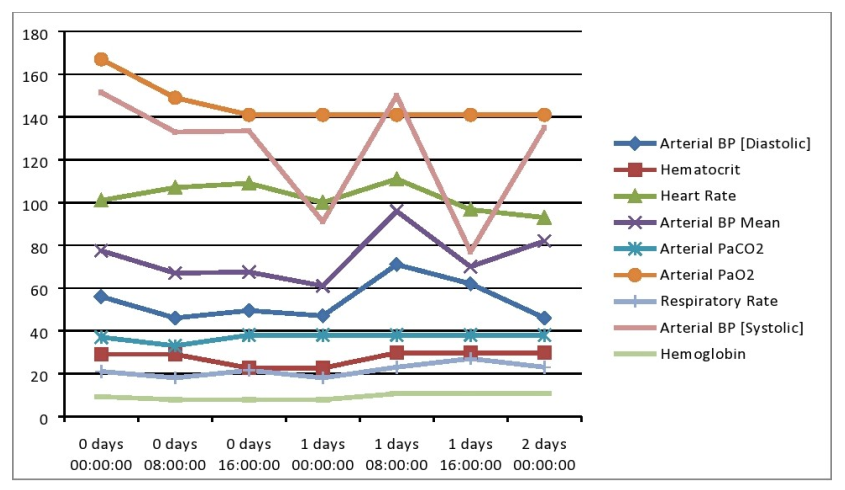
\includegraphics[width=7in,height=4in]{mimic.png}
    \caption{Some of the Clinical recordings associated with each patient[\citenum{johnson2016mimic}]}
    \label{fig:mimic-iii}
\end{figure}
\subsection{Data Preprocessing}
\subsubsection{Data Extraction}
MIMIC-III dataset consisted of around 58,576 patients who were diagnosed as suffering from different types of disease and hence mortality due to those diseases.  These diseases include Pulmonary disease, Circulatory disease, Trauma, a disease of the digestive system and many more.  Since the dataset is very large, we only consider data of those patients who were readmitted again which gives the details of 7,534  patients.   The data set is divided into two classes:-
\begin{itemize}
    \item Patients readmitted in 30 days.
    \item Patients readmitted after 30 days.
\end{itemize}


\subsubsection{Missing Values}
MIMIC-III  dataset contains missing values in some of the features.   The feature will  be removed if it contains more missing value otherwise mean will be used to fill the missing values.

\subsubsection{Normalization}
Normalization is used to remove the biases among the features.   It brings the data on a standard scale.  It standardizes the range of independent features or variables of data, called feature scaling.

\subsection{Feature Selection}
Features are selected through Nature Inspired Algorithms:
\subsubsection{Bat Algorithm}
Bat Algorithm is an optimization algorithm inspired by the echolocation behavior of microbats[\citenum{yang2012bat}].  Bats uses echolocation to sense distance, and they also distinguish be-tween food/prey and other background barriers.  Bats fly randomly with velocity $v_i$ at location $x_i$ with a fixed frequency $f_{min}$, varying wavelength and loudness $A_0$ to search for the victim.  They can automatically regulate the wavelength (or frequency) of their emitted pulses and adjust the rate of pulse emission r in the scale of [0, 1], depending on the closeness of their target. Although  the  loudness  can  diversify  in  many  ways,  we  assume  that  the  loudness  varies  from  a high (positive) $A_0$ to a minimum constant value $A_{min}$.
Rules to update position $x_i$ and velocity $v_i$ of bats at time step t is given by:
\begin{equation}
    f_i = f_{min} + (f_{max}-f_{min})\beta
\end{equation}
\begin{equation}
    v^t_i = v^{t-1}_i+(x^{t-1}_i-x_b)f_i
\end{equation}
\begin{equation}
    x^t_i = x^{t-1}_i+v^t_i
\end{equation}
where $\beta\in$[0,1]  is  a  random  vector  drawn  from  a  uniform  distribution and $x_{b}$ is the current global best solution  which is found after comparing all the solutions among all  the n bats.
For the local search part once a solution is selected among the current best solutions, a new solution for each bat is generated locally using a local random walk:
\begin{equation}
    x_{new} = x_{old} + \epsilon A^t
\end{equation}
where $\epsilon \in$[-1,1] is a random number. $A^t$ is the average loudness of all the bats at that time step.\\
Variation of Loudness and Pulse Emission:
\begin{equation}
    A^{t+1}_i = \alpha A^t_i
\end{equation}
\begin{equation}
    r^{t+1}_i = r^0_i [1-exp(-\gamma t)]
\end{equation}
where $\alpha$ \& $\gamma$  are constant.
\subsubsection{Grey Wolf Optimizer}
Grey Wolf Optimizer (GWO) Algorithm inspired by grey wolves[\citenum{mirjalili2014grey}]. The GWO algorithm mimics the leadership hierarchy and hunting mechanism of grey wolves in nature. Four types of grey wolves are employed for simulating the leadership hierarchy such as alpha, beta, delta, and omega. Also, the three main steps of hunting, searching for prey, encircling prey, and attacking victim, are implemented.\\
Alpha wolf is a leader male or female. They make decisions like the sleeping place, hunting, etc. Other wolves acknowledge alpha wolf by their tail down. Beta wolf help alpha wolf in making decisions. They are an advisor for alpha and discipliner for the pack. They also ensure all subordinate obey the order of alpha and give feedback to alpha. Delta wolves also called subordinate. They dominate omega wolves.\\
Categories of Delta wolves:-
\begin{itemize}
    \item Scouts - Watch boundaries.
    \item Sentinels - Protect pack.
    \item Elders - Aplha or beta wolf sometimes.
    \item Hunters - Help aplha and beta wolf in hunting.
    \item Care Taker - Care ill weak and wounded wolves.
\end{itemize}
Omega wolves are like the scapegoat in the pack. They are last allowed wolves to eat having weak fitness.\\
Search Process in GWO Algorithm:-
\begin{itemize}
    \item Searching
    \item Encircling
    \item Attacking the prey
\end{itemize}

\paragraph{Searching}
\begin{itemize}
    \item Search according to aplha, beta and delta wolves. They diverge to search for prey and converge to attack prey.
    \item Modeled by utilizing A random variable greater than 1 or less than -1.
    \item When $|A| >$ 1 wolves are forced to diverge from prey to find better solution.
\end{itemize}
\paragraph{Encircling Prey}
It is the process in which wolves encircle the prey for attack. It is modeled as:
\begin{equation}
    \overrightarrow{\text{D}} = |\overrightarrow{\text{C} }\overrightarrow{\text{X}}_p(t)  - \overrightarrow{\text{X}}(t)|
\end{equation}
\begin{equation}
    \overrightarrow{\text{X}}(t+1) = \overrightarrow{\text{X}}_p(t) - \overrightarrow{\text{A}}\overrightarrow{\text{D}}
\end{equation}
Where t is the current iteration, $\overrightarrow{\text{A}}$ , $\overrightarrow{\text{C}}$ are coefficient vectors and $\overrightarrow{\text{X}}_p$ is position of prey and $\overrightarrow{\text{X}}$ is the position of grey wolf.\\ \\
\textbf{Updation of Coefficients}
\begin{equation}
    \overrightarrow{\text{A}} = 2\overrightarrow{\text{a}}\overrightarrow{\text{r1}} - \overrightarrow{\text{a}}
\end{equation}
\begin{equation}
    \overrightarrow{\text{C}} = 2\overrightarrow{\text{r2}}
\end{equation}
Where $\overrightarrow{\text{a}}$ linearly decrease from 2 to 0 over the course of iteration. $\overrightarrow{\text{r1}}$ and $\overrightarrow{\text{r2}}$ are random vectors $\in$ [0,1].
\paragraph{Attacking}
The hunt is usually guided by alpha. The beta and delta might also participate in hunting. We first save three best solutions i.e. alpha beta and delta which are the best solutions and update positions of other agents based on these three. It is modeled as:
\begin{equation}
    \overrightarrow{\text{D}}_\alpha = |\overrightarrow{\text{C}}_1 \overrightarrow{\text{X}}_\alpha - \overrightarrow{\text{X}}|
\end{equation}
\begin{equation}
    \overrightarrow{\text{D}}_\beta = |\overrightarrow{\text{C}}_2 \overrightarrow{\text{X}}_\beta - \overrightarrow{\text{X}}|
\end{equation}
\begin{equation}
    \overrightarrow{\text{D}}_\delta = |\overrightarrow{\text{C}}_3 \overrightarrow{\text{X}}_\delta - \overrightarrow{\text{X}}|
\end{equation}
\begin{equation}
    \overrightarrow{\text{X}}_1 = \overrightarrow{\text{X}}_\alpha - \overrightarrow{\text{A}}_1 \overrightarrow{\text{D}}_\alpha
\end{equation}
\begin{equation}
    \overrightarrow{\text{X}}_2 = \overrightarrow{\text{X}}_\beta - \overrightarrow{\text{A}}_2 \overrightarrow{\text{D}}_\beta
\end{equation}
\begin{equation}
    \overrightarrow{\text{X}}_3 = \overrightarrow{\text{X}}_\delta - \overrightarrow{\text{A}}_3 \overrightarrow{\text{D}}_\delta
\end{equation}
\begin{equation}
    \overrightarrow{\text{X}}(t+1) = (\overrightarrow{\text{X}}_1 + \overrightarrow{\text{X}}_2 + \overrightarrow{\text{X}}_3) / 3
\end{equation}
Grey wolf attack prey when it stops moving. In GWO vector A is a random value within an interval [-2a,2a] a decrease from 2 to 0 throughout the iteration. When $|A|<1$ wolves attack prey.

\subsection{Feature Extraction}
For feature extraction Convolution Neural Network(CNN) is used.
\subsubsection{Convolutional Neural Network}
Convolutional neural network is an effective machine learning technique from the deep learning and it is similar to ordinary Neural Networks. Convolutional neural network is a network with convolutional layers. Convolutional neural network is consists of three steps of neural layers to build its architectures: Convolutional, Pooling, and Fully-Connected.\\ \newline
\textbf{Convolutional layers:}
		The convolutional layer is the main part of the convolutional neural network. In the convolutional layer the output result is derived from the input by filtering in certain conditions.
		Convolutional layers consist of a rectangular grid or cubic block of neurons. It means input, output layers with filters can be a rectangular grid or cubic block of neurons.\\
		
		The filter is supplied from uppermost left to downside right. In every location of the filter, the weighted volume of the pixels is determined by the equation \begin{equation}WT^X + b\end{equation}and a new neuron is acquired.
		In the convolutional layer three kind of hyper parameters determine the volume of the output neurons: depth, stride, and zero-padding.
		A number of the filters with certain strides determines the depth For original RGB image depth equal to three.

		Here, whereas the stride equal to 1, the filters runs a single pixel. In this case output neuron is 5x5xd. Whereas the stride equal to 2, the filters are skipped two pixels and output neuron size is 3x3xd. In the last case, when stride is 3 the filters are skipped 3 pixels. Output neuron size is 2x2xd.
		
		Zero padding is the filling process in the input neuron where it zeros are around the edge. Zero-padding is mostly consumed for adjustment the size of the input neuron for research purposes. It is normally applied for when the input neuron size needs to maintain in the output neuron.The output neuron size is calculated by equation \\
	    \begin{equation}Output = (W-K+2P)/S+1\end{equation}
	    where W is the input neuron’s size, K is the filter (kernel) size, P is size of the padding, and S is the stride.
	    In the convolutional neural network linear algebraic operations are also used. Suppose that matrix dimensions are m and n (m rows, n columns). 2D convolutional cube calculates the two-dimensional convolution with two input matrices. (MA, NA) is dimensions of the matrix A, and (MB, NB) is dimensions for the matrix B. In case, the cube determines the complete output size, convolution equation is as below 
	    \begin{equation}C(i,j)=\sum^{{M_A}- 1}_{m=0}\sum^{{N_A}- 1}_{n=0}A(m,n)*B(i-m,j-n)\end{equation}
\textbf{Max-pooling layer:}	After each convolutional layer, a pooling layer executes next operation. The pooling layers are utilized to decrease size of the input neuron. This layer acquires small rectangular blocks from the convolutional layer and samples it to provide a single output from that block. The max pooling method is common used. A formulation for a single type of the pooling layer, max-pooling is presented in equation \begin{equation}
    h_l^j(x,y)=max  \in \mathcal{N}(x),y \in \mathcal{N}(y)h^{l-1}_j(\bar{x},\bar{y})
\end{equation}\\ \\
\textbf{Fully Connected layers:} Fully connected layer is the last layer, which is constructed from connection of all previous neurons. The fully connected layer normally promotes reduction of spatial information because it “fully connected”: from all input neurons until all output neurons.


\subsection{Algorithms}

\subsubsection{Recurrent Neural Network}
Recurrent neural networks (RNN) are used to capture the temporal dependency in the time series data[\citenum{che2018recurrent}]. As most of the healthcare data is a series of temporal recordings, hence RNNs have been widely adopted in the healthcare domain. We are usually provided with a series of observations $x_1$...$x_T$ and we train a classifier to generate hypotheses \^{y}. The recurrent connections are added in feed-forward neural networks to make it RNN. The output of a neuron in a typical NN is as follows:
    
    \begin{equation}
        y^t_i = \sigma(W_i x^t + b_i)
    \end{equation}
Where $W_i$ is the weight matrix, bi is the bias and represents the sigmoid function. While in the case of RNN, a neuron is fed with the output of the neuron at time t-1.  The following equation shows the new activation function:
    \begin{equation}
        y_i^t = \sigmoid(W_i x^t + V_i x^{t-1} + b_i)
    \end{equation}
As  RNN uses the previous outputs as recurrent connection, their current output depends upon the previous states.  This property of RNN makes it very useful in sequence labeling tasks. The backpropagation through time can be used to train RNNs. It was demonstrated by that learning long-term dependencies is difficult using gradient descent. This is mainly because the backpropagating error can vanish which makes the network inefficient in learning long-range dependencies, or frequently explode which makes convergence impossible.\\
LSTM networks were proposed to tackle the problem of vanishing gradients and were developed to model long-range dependencies efficiently. LSTMs can accomplish this by keeping an internal state that represents the memory cell of the LSTM neuron. This internal state can only be written and read through gates which control the information flowing through the cell state.  The following diagram shows the recurrent neural network.
\begin{figure}[h]
    \centering
    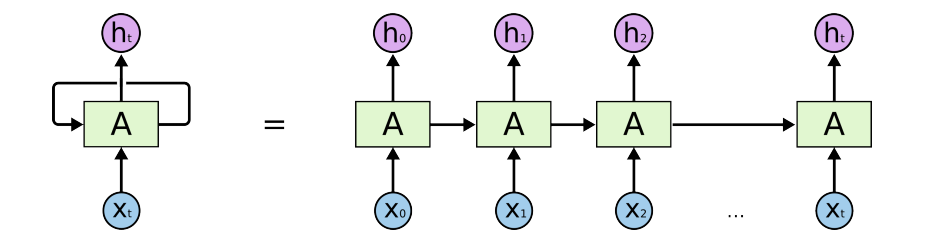
\includegraphics[width=4.1in,height=2in]{rnn.png}
    \caption{An unrolled recurrent neural network[\citenum{greff2017lstm}]}
    \label{fig:rnn}
\end{figure}
\subsubsection{Long Short Term Memory (LSTM) Networks}
Long Short Term Memory networks usually just called LSTMs are a special kind of RNN,
capable of learning long-term dependencies. They were introduced by [\citenum{hochreiter1997long}] and were refined and
popularized by many people. They work remarkably well on a large variety of problems and are
now widely used. To solve long-term dependency problem, LSTMs are explicitly designed. Remembering information for long periods of time is practically their default behavior, not something
they struggle to learn! All recurrent neural networks have the form of a chain of repeating modules
of the neural network. In traditional RNNs, this repeating module will have a pretty simple structure, such
as a single tank layer. LSTMs also have this chain-like structure, but the recurrent module has a
different structure. Rather than having a single neural network layer, there are four layers which are interacting extraordinarily.   The intermediate information is stored in a single hidden layer h and its state
changes over time ($h_{t-1}$, $h_{t}$, $h_{t+1}$). On the final hidden state vector $h_{T}$, we used a fully connected
layer followed by sigmoid function. For loss function, we used log loss. The following equations can be used for calculation of the current hidden layer $h_{t}$.
\begin{equation}
    f_t = \sigma(W_fX_t + R_fh_{t-1} + b_f )
\end{equation}
\begin{equation}
    i_t = \sigma(W_iX_t + R_ih_{t-1} + b_i)
\end{equation}

\begin{equation}
    o_t = \sigma(W_o X_t + R_oh_{t-1} + b_o)
\end{equation}
    
\begin{equation}
    \tilde{C}_t = \Phi(W_C X_t + R_C h_{t-1} + b_c) 
\end{equation}

\begin{equation}
    C_t = f_t C_{t-1} + i_t \tilde{C}_t 
\end{equation}

\begin{equation}
    h_t = o_t\phi(C_t)
\end{equation}
$f_t$ , $i_t$ and $o_t$ are forget gate, input gate and output gate respectively. To decide which
historical information will be discarded from the cell state forget gates are used, the update of
cell state is decided by the input gate, and the output
gate decides the output of the cell state. Cell states are completely overridden in classical RNN, but LSTM has the potential to add
or remove information to the cell state. The input weight of each gate, recurrent weight, and the
bias are expressed as W* , R* , b*  respectively where * can be f, i, o and c. Here $\sigma$, $\Phi$ stands
for an element-wise application of the sigmoid (logistic) and tanh function respectively. For matrix
multiplication. The candidate values are computed in equation (6), and equation(7) old state
is multiplied by $f_t$, and this helps in forgetting the things we decided to forget. Then $i_t$*$\delta C_t$ is
added in it. This is the new candidate values, scaled by how much we decided to update each state
value. The final output of an LSTM unit is given by equation 8. Here * represents the Hadamard
(element-wise) multiplication operation. Figure 3 shows the LSTM network.
\begin{figure}[h]
    \centering
    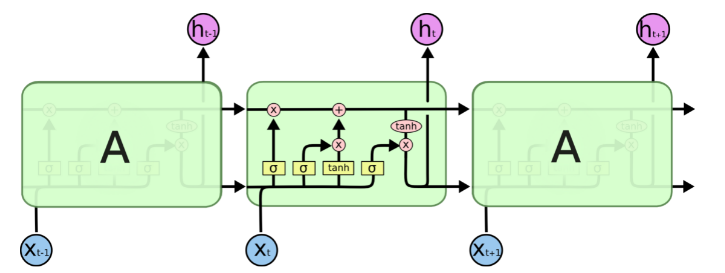
\includegraphics[width=5in]{lstm.png}
    \caption{The repeating module in an LSTM contains four interacting layers[\citenum{greff2017lstm}]}
    \label{fig:lstm}
\end{figure}

\subsubsection{Bidirectional Recurrent Neural Networks (BRNN)}
Bidirectional Recurrent Neural Networks also called BRNN is just like RNN but it trains simultaneously on both sides of the time series data[\citenum{schuster1997bidirectional}]. This model gives the better result in both regression and classification problem. BRNN computes both forward $(\overrightarrow{\text{h}})$ and backward $(\overleftarrow{\text{h}})$ hidden sequence.
\begin{equation}
    \overrightarrow{\text{h}}_t = \mathcal{H}(W_{x\overrightarrow{\text{h}}} x_t + W_{\overrightarrow{\text{h}} \overrightarrow{\text{h}}} \overrightarrow{\text{h}}_{t-1} + b_{\overrightarrow{\text{h}}})
\end{equation}
\begin{equation}
    \overleftarrow{\text{h}}_t = \mathcal{H}(W_{x\overleftarrow{\text{h}}} x_t + W_{\overleftarrow{\text{h}} \overleftarrow{\text{h}}} \overleftarrow{\text{h}}_{t+1} + b_{\overleftarrow{\text{h}}})
\end{equation}

\begin{equation}
    y_t = W_{\overrightarrow{\text{h}}y}\overrightarrow{\text{h}}_t + W_{\overleftarrow{\text{h}}y}\overleftarrow{\text{h}}_t +b_o
\end{equation}
The long range context can be accessed in both directions by combining BRNNs with LSTM which gives bidirectional LSTM[\citenum{graves2005framewise}].

\begin{figure}[h]
    \centering
    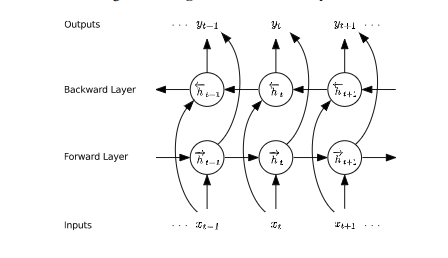
\includegraphics[width=7in, height=2.5in]{brnn.png}
    \caption{Bidirectional Recurrent Neural Networks[\citenum{graves2014towards}]}
    \label{fig:brnn}
\end{figure}
\newpage

\subsubsection{Auto Encoders}
An auto-encoder is a neural network model that seeks to learn a compressed representation of an input.
They are an unsupervised learning method, although technically, they are trained using supervised learning methods, referred to as self-supervised. They are typically trained as part of a broader model that attempts to recreate the input.
The design of the auto-encoder model purposefully makes this challenging by restricting the architecture to a bottleneck at the midpoint of the model, from which the reconstruction of the input data is performed.
In this case, once the model is fit, the reconstruction aspect of the model can be discarded and the model up to the point of the bottleneck can be used. The output of the model at the bottleneck is a fixed length vector that provides a compressed representation of the input data.
Input data from the domain can then be provided to the model and the output of the model at the bottleneck can be used as a feature vector in a supervised learning model, for visualization, or more generally for dimensionality reduction.
\newpage
\subsection{Flow Diagram}
\begin{figure}[h]
    \centering
    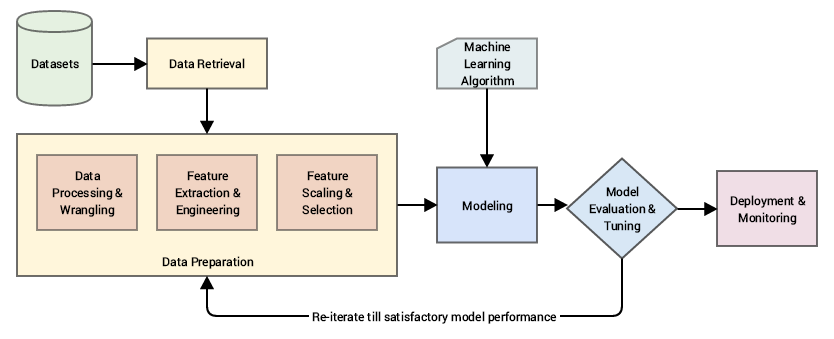
\includegraphics[width=6.5in]{flowdiag.png}
    \caption{Flow Diagram}
    \label{fig:flowdiag}
\end{figure}
\subsection{Implementation Details}
The entire dataset was split using stratified sampling and 10\% of the dataset was used as a validation set and random search was used for hyperparameter optimization. The rest 80\% of the dataset was used for training purpose and was tested on 10\% of the dataset. The LSTM model was trained with 30 epochs using Adam optimizer. LSTM layer uses 100 memory cell with no dropout and 25 memory cell with 20\% dropout and these architectures are found after validation performance. Also train this model with Bat Algorithm.
\\
Another model train on this dataset was convolution long short term memory(CLSTM). It is a hybrid model in which convolution layers are used for feature extraction. The CLSTM model was trained with 30 epochs and the batch size of 1000. First, the convolution layer was used with 45 filters of size $5\times5$. Then the LSTM layer that uses 100 memory cell with 20\% dropout. Also train this model with Grey Wolf Optimizer Algorithm.\\
In the training phase, the model was saved and also compute these performance metrics (AUC, F1, precision, and recall).\\
Several built-in modules of python will be utilized, namely:
\begin{itemize}
    \item Numpy
    \item Pandas
    \item Scikit-Learn
    \item Keras
    \item Matplotlib
    \item NiaPy
\end{itemize}
The computations were performed on Ubuntu 16.04 LTS with following hardware specifications:
\begin{itemize}
    \item \textbf{Processor} Intel i7 6th Gen. broadwalle processor.
    \item \textbf{RAM} 24 GB DDR4
    \item \textbf{Secondary Memory} 250 GB SSD
    \item \textbf{Graphics Card} Nvidia 1080Ti 11GB
\end{itemize}
\subsection{Preliminary Testing and Results Obtained}
This section presents the readmission prediction results obtained from different predictive models. The prediction accuracy will be compared in terms of two factors AUC under ROC (Receiver Operating Characteristic) Curve[\citenum{je2005formulation}], and overall accuracy. Both area under ROC curve and overall accuracy
depends on the classifier’s ability to rank patterns for positive class, but in the case of overall accuracy, it also depends on the ability to calculate the threshold in the ranking to classify the positive class. Applying different algorithms on the dataset, with default parameters, we obtained results we obtained results as mentioned in Table 1.
\begin{table}[h]
\centering
\begin{tabular}{ p{5cm} | c | p{2cm}}
Methods & Area Under ROC Curve & Accuracy\\
\hline \hline
Long Short Term Memory & 0.79 & 79.84\%\\
\hline
Long Short Term Memory Auto-Encoders & 0.73 & 70.00\%\\
\hline
Convolution Long Short Term Memory & 0.75 & 70.98\%\\
\hline
Long Short Term Memory with Bat Algorithm & 0.75 & 70.42\%\\
\hline
Long Short Term Memory with Grey Wolf optimizer Algorithm & 0.85 & 81.57\%\\
\hline
Long Short Term Memory with Bat Algorithm & 0.87 & 80.32\%\\
\hline
Convolution Long Short Term  Memory  Auto-Encoders & 0.85 & 77.99\%\\
\hline
\end{tabular}
\caption{Comparison among different Models implemented so far}
\label{tab:tri}
\end{table}

\begin{table}[h]
\centering
\begin{tabular}{ p{5cm} | c | p{2cm}}
Methods & Area Under ROC Curve & Accuracy\\
\hline \hline
Logistic Regression & 0.54 & 58.09\%\\
\hline
Support Vector Machines & 0.54 & 59.37\%\\
\hline
Decision Tree & 0.52 & 55.68\%\\
\hline
Random Forest & 0.53 & 60.49\%\\
\hline
\end{tabular}
\caption{Comparison with Baseline Models}
\label{tab:tri}
\end{table}

\subsubsection{Curves showing Receiver Operating Curve (ROC) of different models}
\begin{figure}[H]
    \centerline{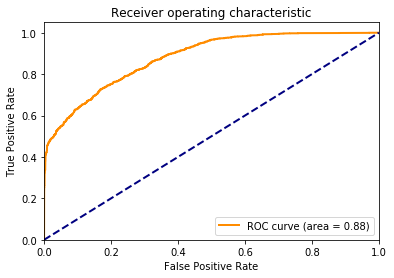
\includegraphics[width=4.5in]{lstm16_4.png}}
    \caption{Receiver Operating Characteristic Curve: Long Short Term Memory.}
\end{figure}
\begin{figure}[H]
    \centerline{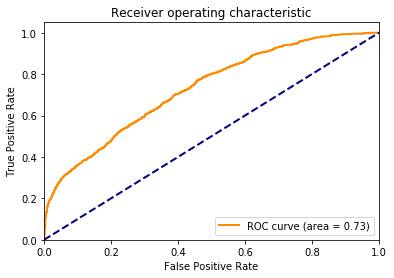
\includegraphics[width=4.5in]{lstm_auto_encoder4.png}}
    \caption{Receiver Operating Characteristic Curve: Long Short Term Memory Auto-Encoders.}
\end{figure}
\begin{figure}[H]
    \centerline{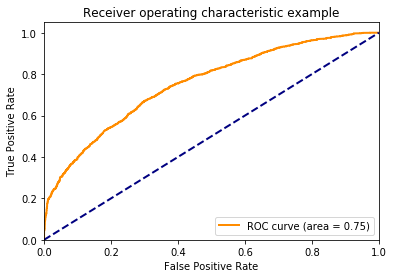
\includegraphics[width=4.5in]{clstm4.png}}
    \caption{Receiver Operating Characteristic Curve: Convolution Long Short Term Memory.}
\end{figure}

\begin{figure}[H]
    \centerline{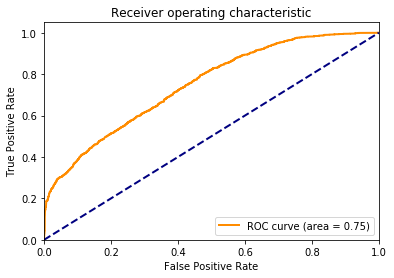
\includegraphics[width=4.5in]{lstm-batalgorithm3.png}}
    \caption{Receiver Operating Characteristic Curve: Long Short Term Memory with Bat Algorithm.}
\end{figure}

\begin{figure}[H]
    \centerline{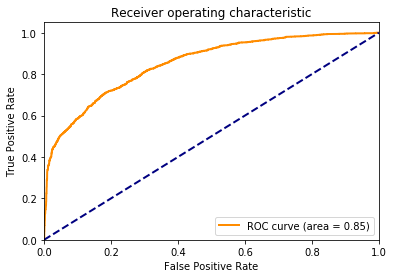
\includegraphics[width=4.5in]{blstm4.png}}
    \caption{Receiver Operating Characteristic Curve: Long Short Term Memory with Grey Wolf Optimizer Algorithm.}
\end{figure}

\begin{figure}[H]
    \centerline{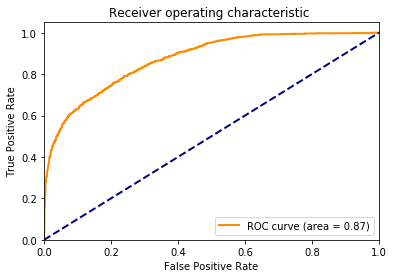
\includegraphics[width=4.5in]{clstm_autoencoder_de4.png}}
    \caption{Receiver Operating Characteristic Curve Convolution Long Short Term Memory Auto Encoders.}
\end{figure}

\begin{figure}[H]
    \centerline{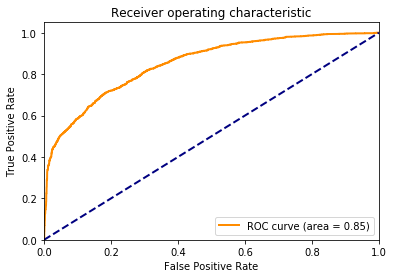
\includegraphics[width=4.5in]{blstm4.png}}
    \caption{Receiver Operating Characteristic Curve Bi-Directional Long Short Term Memory.}
\end{figure}

\section{Expected Results}
\begin{itemize}
    \item To compare the performance of various deep learning models on MIMIC-III dataset based on accuracy and area under roc curve.
    \item Compare the results of deep learning models with baseline models to point the advantages of deep learning in field of health-care applications.
    \item Comparison of results from this thesis with the existing algorithms applied on this dataset.
\end{itemize}


%%%%%%%%%%%%%%%%%%%%%%%%%%%%%%%%%%%%%%%%%
\setcitestyle{numbers}
\setlinespacing{1}
\bibliographystyle{kluwer}
\newpage
\bibliography{my}
\end{document}
